% !TEX root = ../main.tex
\chapter{Semantic Web}
\label{ch:semantic_web}

\nocite{rdf_introduction}
In this chapater will follow a brief description of the concept of ontology and of Semantic Web as defined by W3C. This chapter will then furter detail the ontologies and metadata schemata used in the thesis project, namely Semantic Sensor Network (SSN) and Brick.
It is to note that the work presented in this thesis is not directly using all of these technologies, but it draws from their key concepts to reach some goals. It is therefore worth to mention such concepts here.

\section{Introduction to the Semantic Web}
Semantic Web is a term that identify an evolution of the web in which every resource available through the web is associated with a semantic meaning. Semantic Web technologies enable people to create data stores on the Web, build vocabularies and write rules for handling data.
Semantic web layers are defined by W3C as:
\begin{itemize}
  \item linked data
  \item vocabularies
  \item query
  \item inference
\end{itemize}

\subsection{Linked data}
Linked Data lies at the heart of what Semantic Web is all about: large scale integration of, and reasoning on, data on the Web. To make the Web of Data a reality, it is important to have the huge amount of data on the Web available in a standard format, reachable and manageable by Semantic Web tools. Furthermore, not only does the Semantic Web need access to data, but relationships among data should be made available, too, to create a Web of Data (as opposed to a sheer collection of datasets). This collection of interrelated datasets on the Web can also be referred to as Linked Data.

\subsubsection{Resource Description Framework} \label{subsec:rdf}
Resource Description Framework (RDF)\cite{rdf_standard} is a description language, which aims to capture the semantic of linked data. The RDF standard is based on several fundamental concepts. The first such concept is ``resource''. Resources are the basic objects, or ``things'', that have to be described in the domain (e.g. rooms, floors, sensors etc.). All resources are identified through a unique, global identifier called the Universal Resource Identifier (URI). In most applications, the URI is the Uniform Resource Locator (URL) of a Web page, a part of a Web page or a link to a document available on a Web server. However, the URI is a more general concept, the only condition is that it uniquely identifies a resource. Examples of resources could be ``unibs:florenzi.002'' as well as ``unibs:thesis1234'' or ``https://www.w3.org/RDF/''.  Another essential concept is ``property''. Properties describe relations between resources and, following the previous example, we could say that ``has\textunderscore author'', ``has\textunderscore name'', ``has\textunderscore subject'' are properties.  Having defined both resources and properties, statements can be derived. Statements, also known as triples, in RDF have the basic form: subject-predicate-object, where the subject is an RDF resource, the predicate is a RDF property, and the object is another RDF resource or a literal (a name, a number, a code, etc.). Still referring to the example, the statements could be ``unibs:thesis1234 has\textunderscore author unibs:florenzi.002'', ``unibs:thesis1234 has\textunderscore subject \url{https://www.w3.org/RDF}'' and ``unibs:florenzi.002 has\textunderscore name ``Fabio Lorenzi''''.
RDF data models end up being represented as graphs where subjects and objects are nodes while properties are edges. The resulting graph derived from the description above is shown in \autoref{fig:rdf_example}.
\begin{figure}
  \centering
  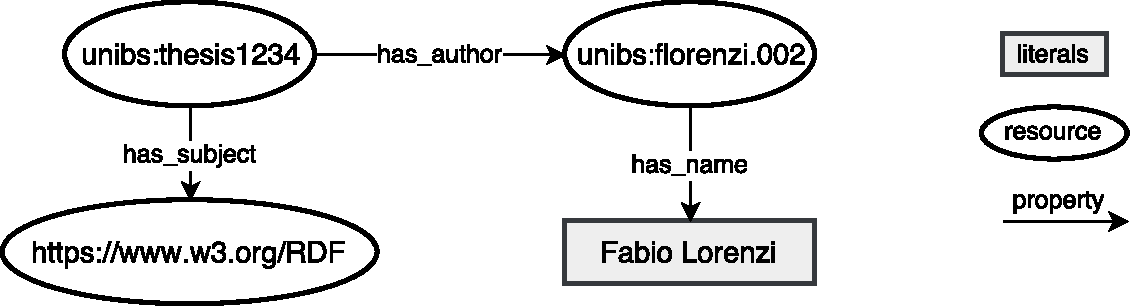
\includegraphics[width=0.8\textwidth]{rdf_example.pdf}
  \caption{Graph representation of the example RDF model}
  \label{fig:rdf_example}
\end{figure}
It is to note that RDF is a conceptual model for representing linked data, but as far as it goes, no semantic is implied in this representation. Looking at this model it is impossible to understand the meaning of the resources or properties, nor to understand if those elements reflect and adhere to rules of a particular domain.
In the example above there is no explicit information telling us that the resource ``unibs:florenzi.002'' is a person and that ``the unibs:thesis1234'' is a book. Furthermore the RDF model represented with ``unibs:florenzi.002 has\textunderscore author unibs:thesis1234'', ``unibs:florenzi.002 has\textunderscore subject \url{https://www.w3.org/RDF}'' and ``unibs:thesis1234   has\textunderscore name ``Fabio Lorenzi'''', yelding the graph representation in \autoref{fig:wrong_rdf_example}, is perfectly fine, altough not semantically correct\footnote{From a common sense point of view. No semantic is actually explicitly declared.}.
Adding semantic to an RDF model, that is detailing the domain ontology, is left to other frameworks as explained in \autoref{subsec:vocabularies}.

\begin{figure}
  \centering
  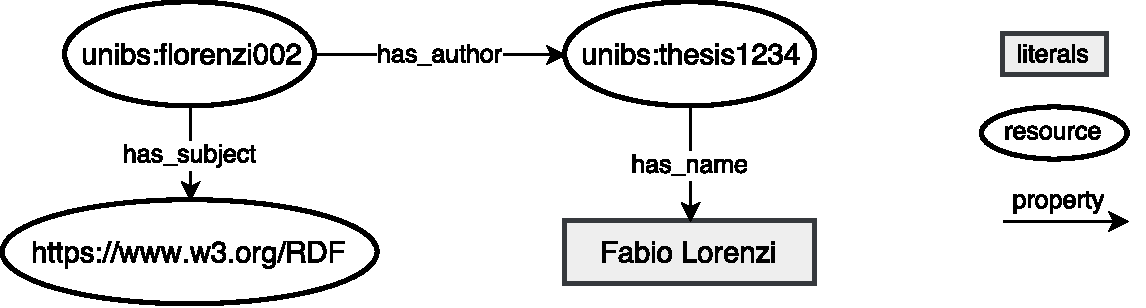
\includegraphics[width=0.8\textwidth]{wrong_rdf_example.pdf}
  \caption{Correct RDF model with wrong semantic}
  \label{fig:wrong_rdf_example}
\end{figure}

\subsection{Vocabularies} \label{subsec:vocabularies}
On the Semantic Web, vocabularies define the concepts and relationships (also referred to as ``terms'') used to describe and represent an area of concern. Vocabularies are used to classify the terms that can be used in a particular application, characterize possible relationships and define possible constraints on using those terms. There is no clear division between what is referred to as ``vocabularies'' and ``ontologies''. The trend is to use the word ``ontology'' for more complex and possibly quite formal collection of terms, whereas ``vocabulary'' is used when such strict formalism is not necessarily used or only in a very loose sense. Vocabularies are the basic building blocks for inference techniques on the Semantic Web.

\subsubsection{Resource Description Framework Schema}
Resource Description Framework Schema (RDFS) defines a set of RDF resources useful for the description of other RDF resources and properties. Through RDFS it is possible to define and detail the semantic of a RDF model. Among the various concepts introduced with RDFS there are:
\begin{itemize}
  \item \textbf{rdfs:Resource}: everything that is described in RDF is a resource
  \item \textbf{rdfs:Literal}: it is a text string
  \item \textbf{rdfs:Property}: it represents the properties
  \item \textbf{rdfs:Class}: it is similar to the concept of type or class in an object oriented programming language
  \item \textbf{rdfs:subClassOf}: it specifies inheritance, eventually multiple, between classes
  \item \textbf{rdfs:range}: it tells which resources are permitted as object in a statement
  \item \textbf{rdfs:domain}: it tells which resources are permitted as subject in a statement.
\end{itemize}
It is to note that the RDFS is a RDF model itself and it is used for explicitly declare the domain knowledge of a given RDF model. We refer to the RDFS as an ontology and to the RDF model triples as the instances of such ontology.
Using RDFS, it is possible to model domain knowledge for the example in \textbf{\autoref{subsec:rdf}} as in \autoref{fig:rdfs_ontology}.
\begin{figure}
  \centering
  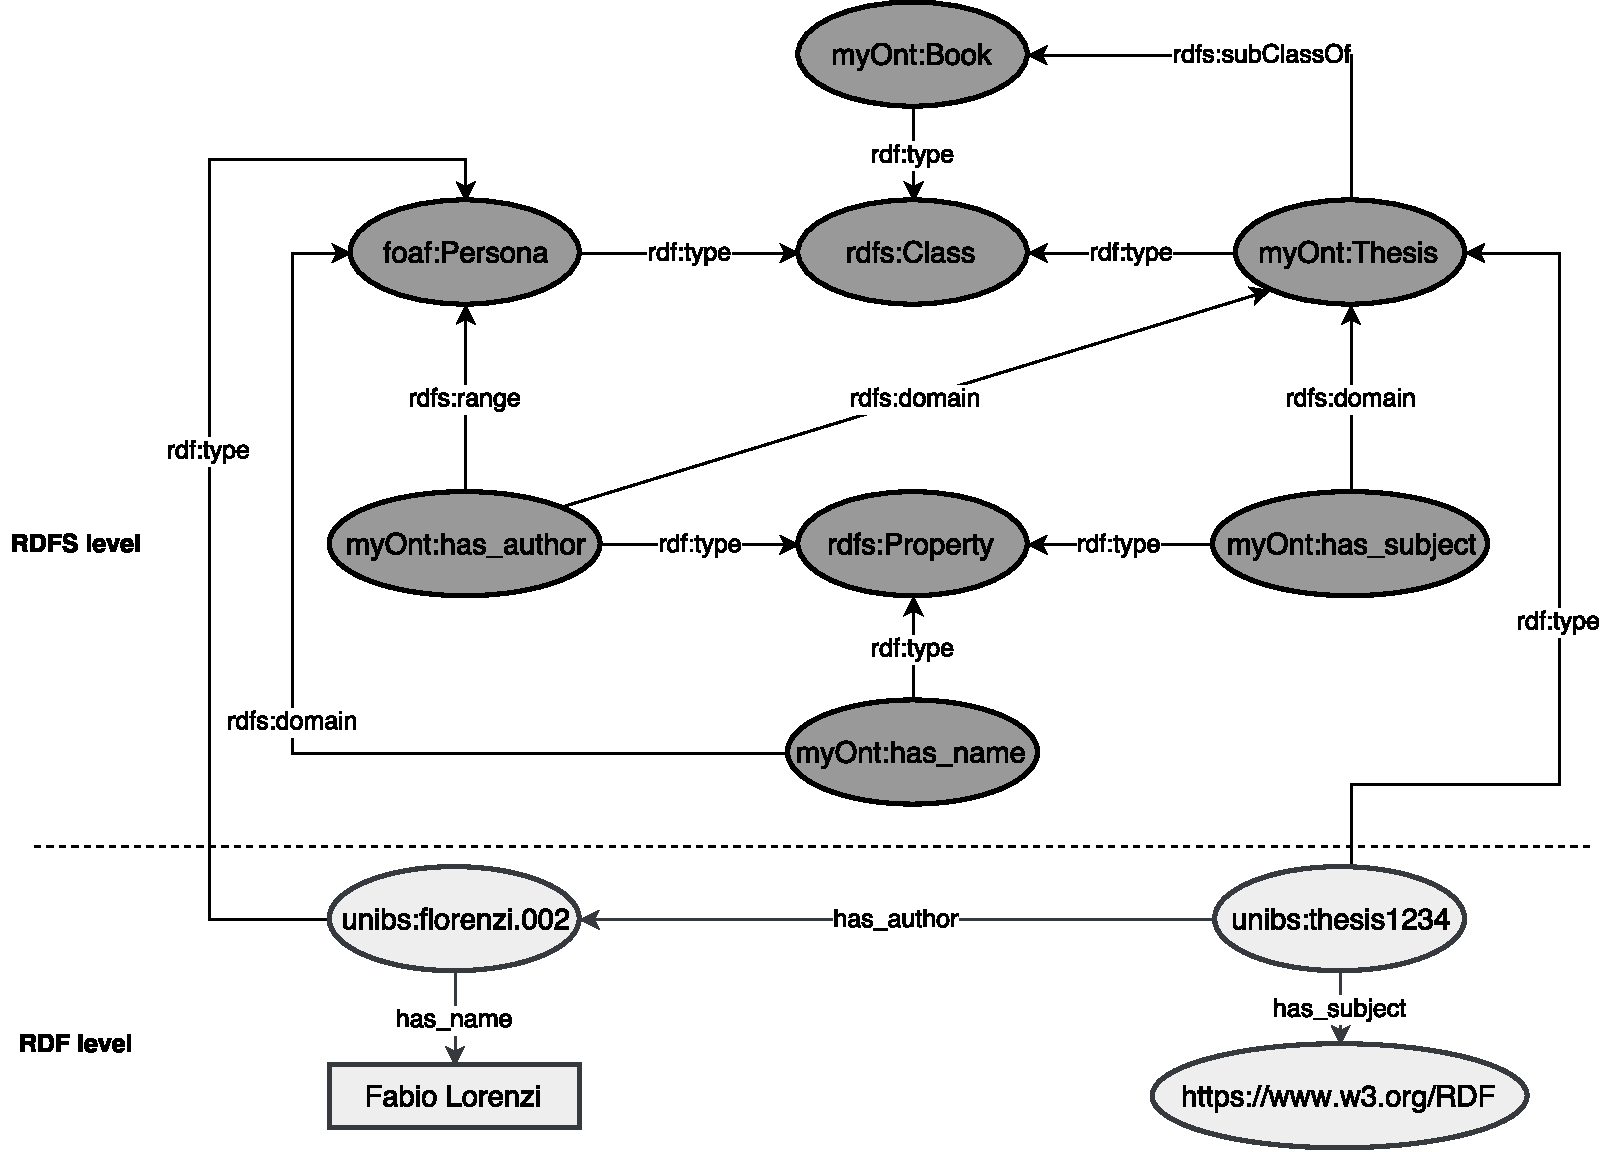
\includegraphics[width=0.9\textwidth]{rdfs_example.pdf}
  \caption{RDFS representation of an ontology}
  \label{fig:rdfs_ontology}
\end{figure}
This ``layering'' approach is what allows for the design of reusable ontologies and gives opportunity to automatically infer new knowledge based on the RDFS model of the data.
Still looking back at the example, lets suppose that the statement ``unibs:florenzi.002 rdf:type foaf:Person'' is not in the ground knowledge of the RDF model. Even if this explicit information wasn't available, a reasoner would have been able to infer that statement (dotted line) given the semantic description of the property ``myOnt:has\textunderscore author'' (bold line). The process is represented in \autoref{fig:inference_rdfs}.
\begin{figure}
  \centering
  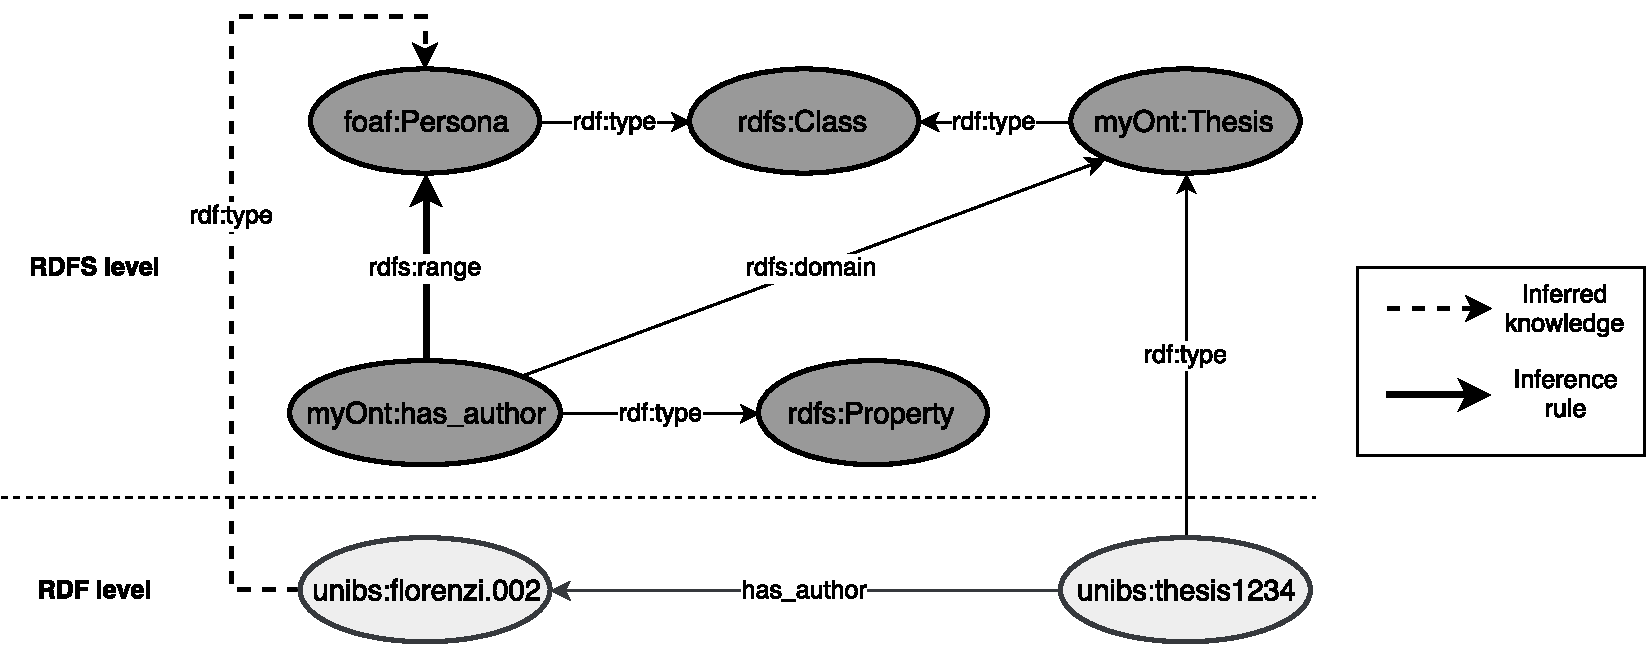
\includegraphics[width=1\textwidth]{inference_rdfs.pdf}
  \caption{Inference process of new knowledge}
  \label{fig:inference_rdfs}
\end{figure}
\subsection{Query}
Since there exist technologies that represent knowledge bases and their semantics, it is useful, if not necessary, to have access to that knowledge through some kind of query language that allows the user to extract and consume that knowledge. If the knowledge base is stored as a RDF, the de-facto standard is represented by SPARQL.

\subsubsection{SPARQL Protocol and RDF Query Language}
A mean for querying RDF models is defined by SPARQL \cite{sparql_reccomendation} query language. SPARQL queries are based on patterns. As RDF can be seen as a set of relationships among resources, SPARQL queries provide one or more patterns against such relationships. A SPARQL engine would perform a pattern matching over the resources and it returns the matching triples. To represent a pattern (or query) to be run against the data model, SPARQL defines a series of keywords similar to those of SQL language:
\begin{itemize}
  \item SELECT followed by the name of the variables that the user wishes to SELECT
  \item INSERT used to insert new triples pattern in the underlying RDF [defined in an extension called SPARQL/Update]
  \item WHERE followed by a set of conditions involving the variable that needs to be selected and that needs to be fulfilled in the underlying RDF.
\end{itemize}
As an example, from \autoref{fig:rdfs_ontology}, a standard query would be to retrieve every thesis and its author in the knwoledge base and it can be written as shown below.
\begin{verbatim}
  SELECT ?thesis ?author
  WHERE
    ?thesis a myOnt:Thesis
    ?thesis has_author ?author
\end{verbatim}


\section{Ontologies for smart buildings}
After the brief (and not exhaustive) introduction to the core concept of the Semantic Web, here are introduced the two main ontologies that lie at the core of the project of this thesis. These ontologies are used to represent a smart building with all its relevant attributes (Brick) and the internal processes that take place involving the building sensors and physic variables (SSN and its extension). Both the ontologies are used since they are ortogonal one another and this help to cover every aspect of interest for a EMS application in a smart building.

\subsection{Brick} \label{subsec:brick}
Brick schema \cite{brick_schema} defines domain specific concepts aimed to describe sensors in a building with its context. It is composed of three parts
\begin{itemize}
  \item a class hierarchy of entities describing various building subsystems
  \item a minimal set of relationships for connecting entities
  \item a method for encapsulation in the form of Function Blocks.
\end{itemize}
The main concept in Brick is the concept of tag introduced with project Haystack \cite{project_haystack}, which is further enriched by an ontology that cristallizes the concepts defined by tags. A tag is a flexible framework for annotating metadata to building data points. In Brick tags are grouped together as sets, named tagsets, to represent entities; the tags {room}, {temperature} and {sensor} can be grouped together as {room temperature sensor} representing a single entity. The concept of tagset is well integrated with the class hierarchy concept of the ontologies: a {room temperature sensor} is a subclass of a generic {temperature sensor}.
As the main goal of Brick is to represent points in a building's BMS, Points is one of the main classes of Brick, which subclasses define specific type of points like Sensor. The most common concepts a Point can be related to are Location, Equipement and Measurement so those classes, together with the Point class, form the core classes of Brick. Those classes are further subclassed to form a hierarchy. A subset of the hierarchy is shown, as an example, in \autoref{fig:brick_hierarchy}.
\begin{figure}
  \centering
  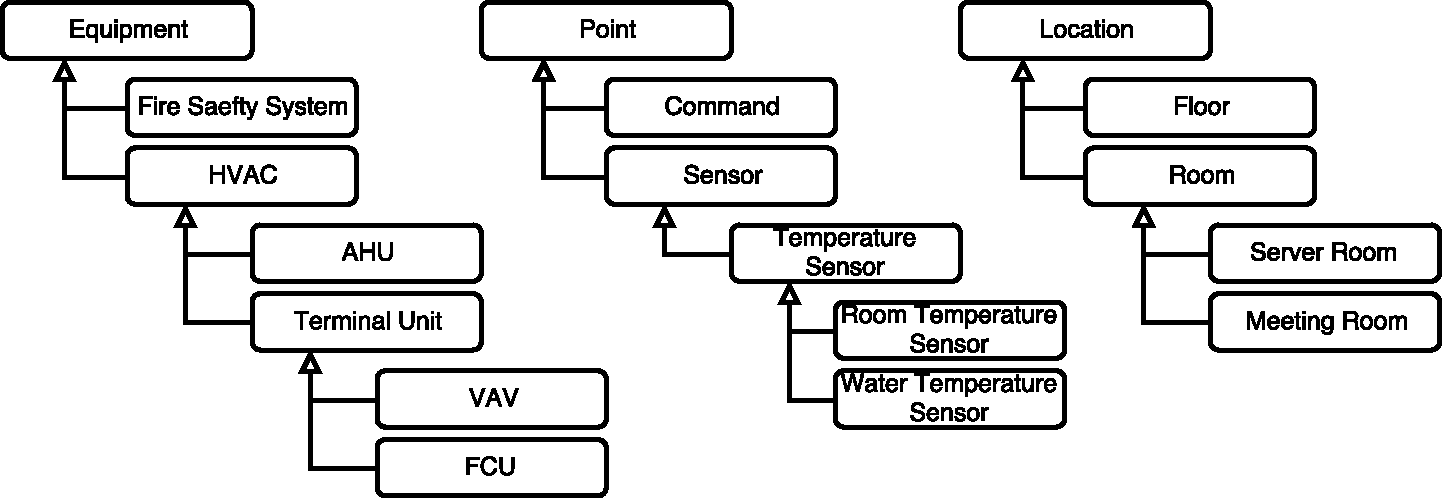
\includegraphics[width=0.9\textwidth]{brick_hierarchy.pdf}
  \caption{Subset of Brick hierarchy}
  \label{fig:brick_hierarchy}
\end{figure}
this taxonomy is able to comprehend almost every entity that can be found in a BMS of a buidling\cite{brick_schema}. Alongside classes, relationships play a crucial role in connecting entities and thus providing a context for many applications. Brick designes a set of minimal, intuitive and multipurpose relationship fundamental in capturing existing relationships in a real building. \autoref{fig:brick_schema} shows the Brick core concepts and the designed set of relationships.
\begin{figure}
  \centering
  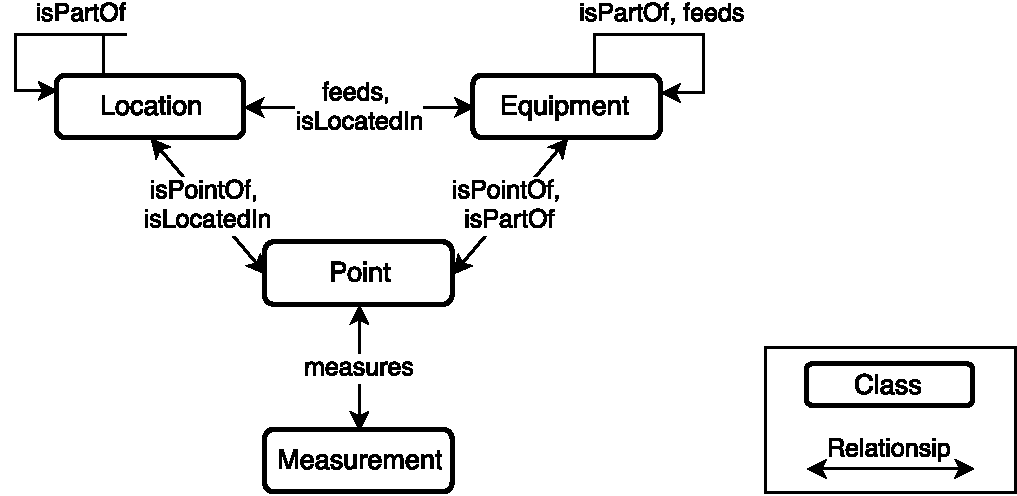
\includegraphics[width=0.7\textwidth]{brick_schema.pdf}
  \caption{Brick schema core concepts}
  \label{fig:brick_schema}
\end{figure}

\subsection{Semantic Sensor Network ontology} \label{subsec:ssn}
While Brick schema is used to model the building domain, the Semantic Sensor Network (SSN) ontology \cite{ssn_ontology} has been chosen because it provides a different view of the various aspect of the sensing process, beyond the specific building domain. Peculiar to the SNN Ontology (SSNO) is the Stimulus-Sensor-Observation design pattern.
This pattern differentiates between the concept of ssn:Sensor for physical devices that take measurements in form of ssn:Observation and ssn:Stimulus that is the actual change in the enviroment that caused a particular observation, so that it is possible to differentiate that stimuli occur in the reality even if no sensor is monitoring them, thus modelling unobservable states of a system, and that observation made from a sensor can be different from the real event (e.g errors, failures, noise ). These concepts aside, SSN provides other useful classes that are ssn:FeatureOfInterest that represents generic entities which status is to be monitored (e.g rooms, fans or floors) and ssn:Property that embodies specific physical quantities that a sensor ought to monitor. All the classes are connected by a set of relationships that are ssn:hasProperty that connects a ssn:FeatureOfInterest with meaningful physical properties, like a temperature in a room; ssn:isProxyFor represents that a given ssn:Stimulus influences a ssn:Property; ssn:includeEvent create a dependency between an observation and an event that causes it; ssn:observedBy links an observation to the sensor that could measure it. \autoref{fig:ssn_ontology} shows the resulting SSN ontology core.

\begin{figure}
  \centering
  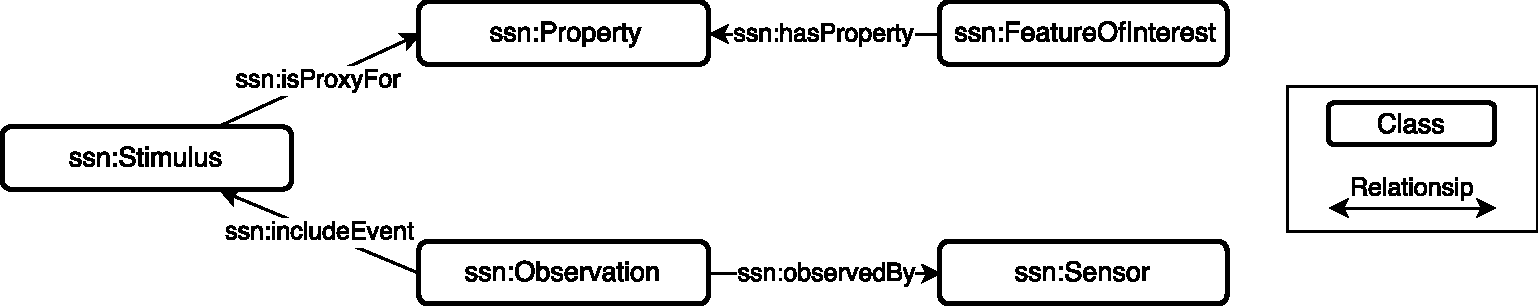
\includegraphics[width=1\textwidth]{ssn_ontology.pdf}
  \caption{Semantic Sensor Network (simplified) ontology}
  \label{fig:ssn_ontology}
\end{figure}

\subsubsection{Extending SSNO} \label{ssubsec:extended_ssno}
As far as it goes, Brick and SSN are good ontologies for modelling a building and its sensor network, but in a Energy Management System (EMS) context, and for FDD applications in particular, it is essential to understand the cause-effect relationships in the building. In order to do that, IBM Research extended the SSNO through the introduction of additional classes and references as in \autoref{fig:extended_ssno}. phy:PhysicalProcess represents laws of physics through a simplified model. Different subclasses of physical processes are derived from LTI system processes and will be described in \autoref{ch:model}.
phy:FeatureLink tells which kind of relationship exists between two ssn:FeatureOfInterest, such a link could be a wall between two rooms or a window between a room and the outside. phy:Cause and phy:Effect are subclasses of ssn:Stimulus useful to differentiate whether said stimulus is a cause or an effect of a ssn:Observation. phy:Anomaly is a subclass of ssn:Observation; it describes out-of-range observations that need to be diagnosed, like a high temperature in a room. phy:ObservedCause is still a subclass of ssn:Observation; it is used for describing a measurment that can be a cause of an anomaly.

\begin{figure}
  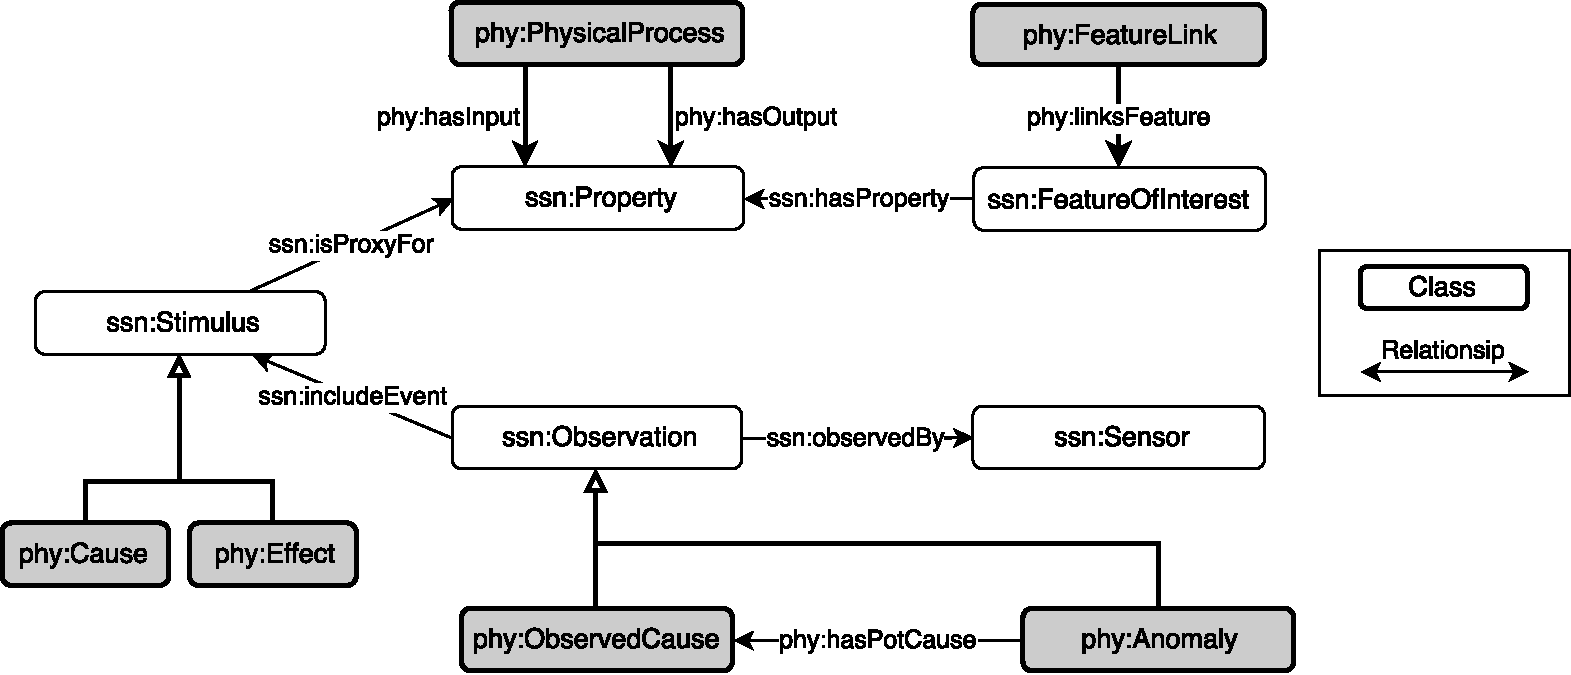
\includegraphics[width=1\textwidth]{extended_ssno.pdf}
  \caption{Extended SSN ontology. Extensions are highlighted with bold line and a light grey background.}
  \label{fig:extended_ssno}
\end{figure}
